\section{Preface}
\label{sec:preface}

In the year 1953, Enrico Fermi, John Pasta, Stanislaw Ulam, and Mary Tsingou conducted computer simulation experiments of a vibrating string that included non-linear terms. Based on some initial assumptions they were expecting the bahvior of this system to have an ergodic properties. And for those who are unfamiliar an ergodic behavior is when a system has the property of when given sufficient time, they impringe on all points in a given space. \cite{Anosov} So while these mathematicians expected some sort of ergodic behavior, they actually ended up getting a \emph{quasi-period} \cite{Quasi} behavior. The following behavior was demonstarted given specific intial values k. 
\begin{figure}[H]
\centering
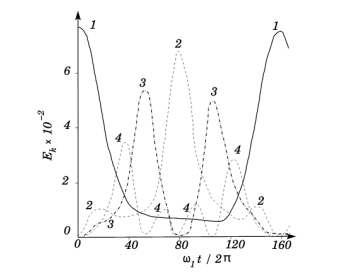
\includegraphics[width=.35\textwidth]{figures/qpb.png}
\caption{The Quasi-Periodic Behavior of the Fermi-Pasta-Ulam-Tsingou Problem}
\end{figure}
Overall the FPUT experiment conducted in 1953 was quite the momentous experiment because it showcased some of of the complexities a nonlinear system can have in terms of its behavior. Also in the context of scientific computing, this experiment was one of the first computer simulations in analyzing these systems. 

\section{Equation Breakdown}

In this section we will discuss the mathematics of \textbf{Figure 1}, and also explain both the linear and nonlinear cases of what the FPUT experiment should do. Like we mentioned in the previous section, we are interested in the bahvior of a system of point masses connected by springs (represented as a particle of strings), and how they move given an initial configuration. This system can be seen as a coupled system of second order differential equations of the form:

\begin{equation}
\label{FPUT system of ODE's}
\begin{cases}
\ddot{x} = f_{i} = K(x_{i+1}-2x_{i}+x_{i-1})(1+\alpha(x_{i+1}-x_{i-1}))\\
x_{i}(0) = x_{i}^{0}\\
\dot{x}_{i}(0) = v_{i}^{0}\\
\end{cases}
\end{equation}
In \textbf{equation 1}, $K$ is the spring constant, $\alpha$ is the strength of the nonlinearity, and $x_{i}(t)$ is the deviation of the $i^{th}$ mass from its equilibrium position. Additionally $x_{i}^{0}$ is the initial displacement of the $i^{th}$ mass, and $v_{i}^{0}$ is the initial velocity of the $i^{th}$ mass. We assume that all masses are normalized to one. These paramters and this system works for an infinite systems of point masses. However we can determine the size of the system and truncate that system to $N$ total masses, so $i=1,...,N$

In order to solve this particular equation second order ODE, we must find a numerical method to solve this. Since computers do not perform calculus, there are methods constructed to help solve these with computation. Therefore in order to advance solutions through time we are able to take the $x^{n}_{i}$ and $x^{n-1}_{i}$ in order to get the next solution. This mechanism is what we call the leapfrog method because we use previous and current solutions to generate a future solution. This solution can be calculated using the following:  $${x}^{n+1}_{i} = f_{i} = K(x_{i+1}-2x_{i}+x_{i-1})(1+\alpha(x_{i+1}-x_{i-1}))$$

It is important to know that this equation that resembles how we advance our solutions through time has a linear and non linear component. In the linear component we set our $\alpha$ to be equal to 0. Doing so we will have a normal behavior where the string of masses will simply oscillate up and down without any surprises. 
\begin{figure}[H]
\centering
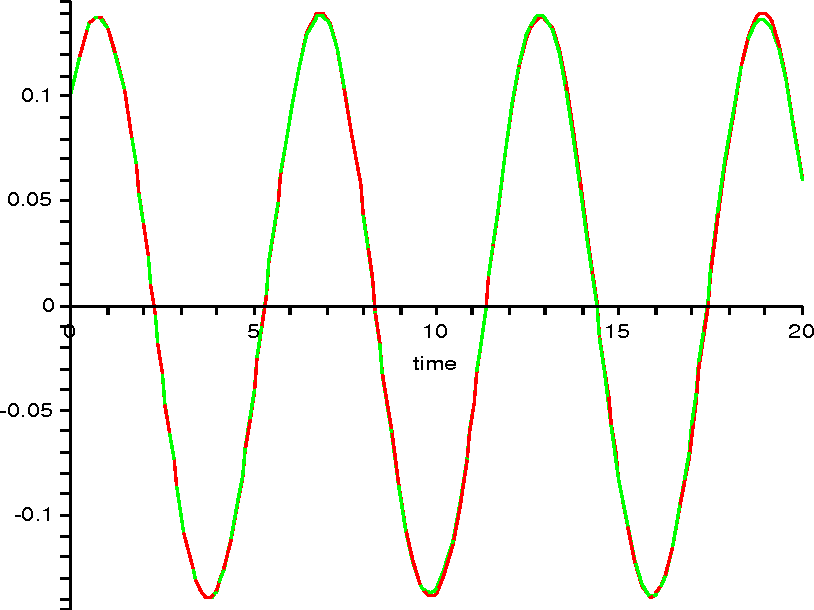
\includegraphics[width=.35\textwidth]{figures/osc-time.png}
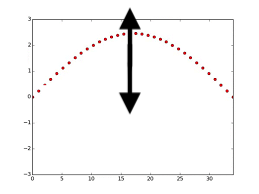
\includegraphics[width=.35\textwidth]{figures/msl.png}
\caption{Oscillating behavior as time moves forward, and representation of string of masses as time moves forward}
\end{figure}

There is nothing obsolete about this behavior, as long as our equation stays linear, the bahvior of the masses on a string will remain consistent. However lets revisit if we include an $\alpha$ value that is not equal to 0. As mentioned in the Preface, Fermi, Pasta, Ulam, and Tsingou thought that the behavior would not follow any certain pattern. However as they ran the simulation they were shocked to find that their was a pattern within this non-linear system. As to why this occurs remains an active part of research but it is odd but amazing how this system in particular behaves.

\section{FPUT implementation}

In the previous section we discussed how these systems were solved numerically through computation. Now that we know the governing equation for this leapfrog method, there are a few architectural designs that we wish to see. The following $x^{n}_{i+1}$, $x^{n}_{i}$, and $x^{n}_{i-1}$ can describe the indeces of an arraand we want to show a high dimensional graphic of what is taking place in this algorithm. 

\begin{figure}[H]
\centering
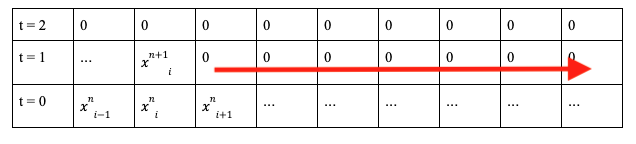
\includegraphics[width=.5\textwidth]{figures/array0.png}
\centering
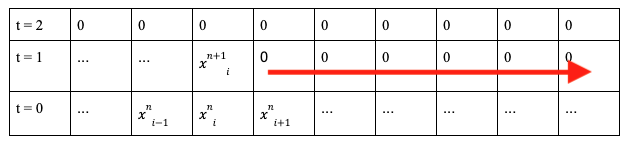
\includegraphics[width=.5\textwidth]{figures/array1.png}
\centering
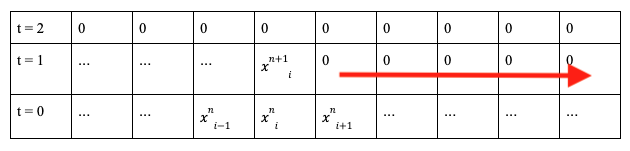
\includegraphics[width=.5\textwidth]{figures/array2.png}
\caption{How the leapfrog method architecture fills in solutions as it advances in time}
\end{figure}

In this graphic we can see how the $x^{n}$ array influences what the solutions of the $x^{n+1}$ arrays will be. And it is also important to note that the solutions get filled from the second index all the way to $N-1$ indeces as there is no way to calculate a $x^{n}_{i-1}$ on the left side and $x^{n}_{i+1}$ on the right side. That is the purpose of the dummy masses that we initialized in \textbf{Equation 1}. So through this represntation we can see specifically how the new solution is generated as we advance through time and how these cells obtain their values. 

In our implementation we can cycle through these arrays by allocating a brand new $x^{n+1}$ array of size $N$ and use a for loop that resembles space to iterate within the interval $1 < x < N-1$ (in a 0 indexed language). After going through the space loop we can follow a specific pattern to continue to advance in time. The pattern can be seen as follows: $$ x^{n-1} = x^{n}$$ $$x^{n} = x^{n+1} $$What this particular means is that $x^{n-1}$ is now timestep 1 and $x^{n}$ is time step 2. This process repeats frequently as long as our time loop keeps iterating.  

\section{Results}
Since the Fermi-Pasta-Ulam-Tsingou problems are still an active field of research, part of this research involves experimenting to see what results we can generate with different number of masses, as well as capturing snapshots at specific time intervals. Specifically we test with $N = {1,8,16,32}$ in terms of different numbers of masses and test at $t=\frac{T_{f}}{4},\frac{T_{f}}{2}, \frac{3T_{f}}{4}, and T_{f}$ time intervals. The following plots are generated showing these different mass numbers and time conditons.

\subsection{Linear-System}

\begin{figure}[h]
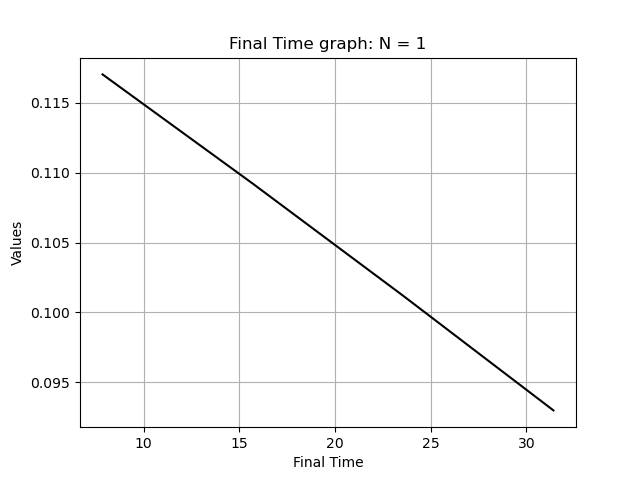
\includegraphics[width=.5\textwidth]{figures/n1mass.png}
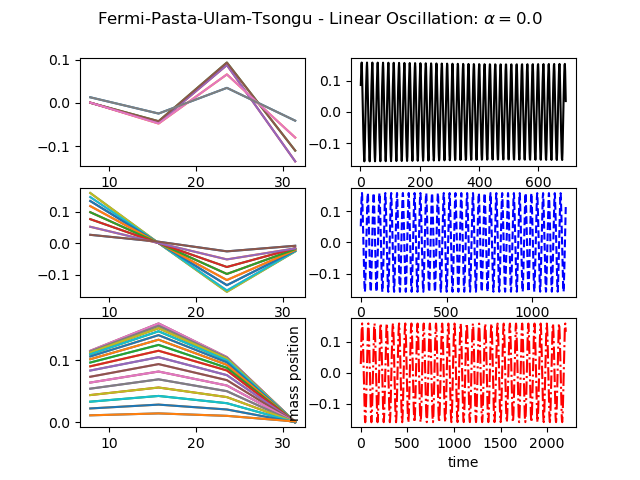
\includegraphics[width=.5\textwidth]{figures/FPUT1.png}
\caption{A plot with 1 mass, as well as a set of subplots of the linear case}
\end{figure}

Lets first examine these two set of plots of the following system. 

\begin{equation}
\label{FPUT system of ODE's}
\begin{cases}
\ddot{x} = f_{i} = K(x_{i+1}-2x_{i}+x_{i-1})\\
x_{i}(0) = x_{i}^{0}\\
\dot{x}_{i}(0) = v_{i}^{0}\\
\end{cases}
\end{equation}

Our first plot as shown in \textbf{Figure 4}, shows our system if we have $N = 1$ mass with no non-linear component. As expected our graph does nothing special as our system simply moves up and down through time. However lets begin to play around with this $N$ variable. Within the subplots displayed in the top right from top to bottom we have the following values for N: 8, 16, 32. Within the subplots we have two columns split into a time graph at points $t=\frac{T_{f}}{4},\frac{T_{f}}{2}, \frac{3T_{f}}{4}, and T_{f}$ time intervals, as well as tracking the mass $i = N/2$ at all time intervals. Through some intial analysis we are not surprised with the overall behavior of $i = N/2$. As expected it oscillates as these sets of string of masses move forward in time. However as we can see in the $N=16, 32$ values, we begin to lose the oscillating structure. My thinking is that these systems move up and down so fast that they construct this weird behavior seen in these graphs. Though very odd, their is also a beauty that we can appreciate from this simulation.  

\subsection{Non-Linear Systems}

\begin{figure}[h]
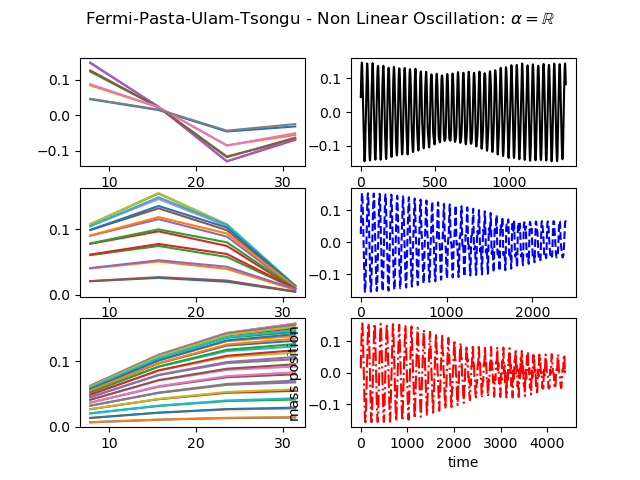
\includegraphics[width=.5\textwidth]{figures/FPUT2.png}
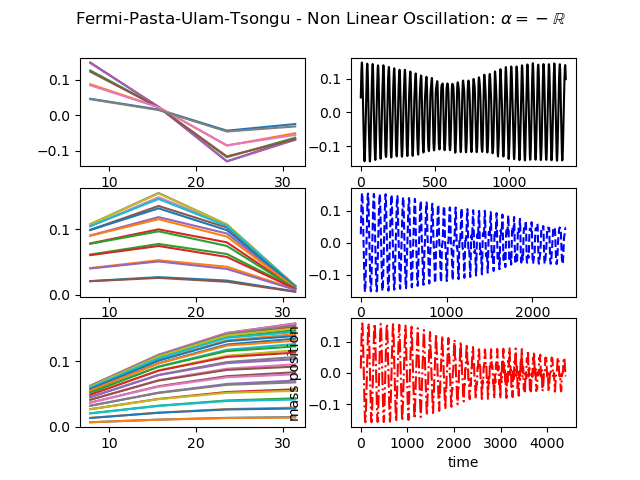
\includegraphics[width=.5\textwidth]{figures/FPUT3.png}
\caption{A set of subplots that show different values of N and how the non-linear constant $\alpha$ affects the system}
\end{figure}

Next we introduce the $\alpha$ constant which was previously described to be the strength of the nonlinearity. What this constant does is introduce a new component to our system as previously shown in \textbf{Equation 1}. By adding the $(1+\alpha(x_{i+1}-x_{i-1})$, there is no surprise that it will affect the overall behavior of the system. One of the big factors that change within this non-linear system is actually the amount of time steps we take. In a linear system we calculated the time step to be the following:

\begin{equation}
\label{FPUT system of ODE's}
M \ge T_{f} \sqrt[2]{K}
\end{equation}

However in a non-linear system we calculate the amount of time steps introducing a new variable $C$ where $C < 1$ which will satisfy us due to the linear version no longer being sufficient for computation. In the following graphs we use the value $C = 0.5$ and it is used to calculate the time step in the following equation: 

\begin{equation}
\label{FPUT system of ODE's}
M = \ceil * {\frac{T_{f} \sqrt[2]{K}}{C}}
\end{equation}
 
So as shown in \textbf{Figure 5}, we see that this system has a "squeeze" affect as for the system with 8 masses. Some implications we can make is that the 16 mass system, as well as the 32 mass system is probably likely going to behave in the same way if our graphs were extended out further. So although the nonlinear constant hardly had an affect on the $t=\frac{T_{f}}{4},\frac{T_{f}}{2}, \frac{3T_{f}}{4}, and T_{f}$ time interval graphs, we can see noticable differences coming from the center mass graph. Another interesting behavior can be seen with the two graphs side by side who have the similar time interval graphs but when it comes to the center mass graph, we can see that system is reflected across the horizontal axis. As we continue our future tests this behavior remains constant.

\subsection{Playing around with the C}

\begin{figure}[h]
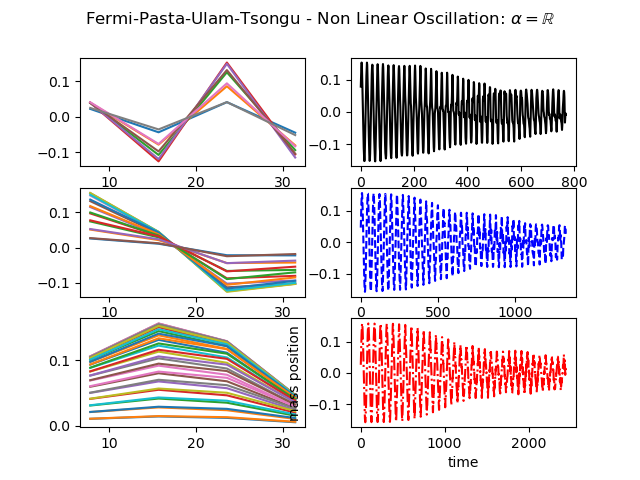
\includegraphics[width=.5\textwidth]{figures/FPUT2.1.png}
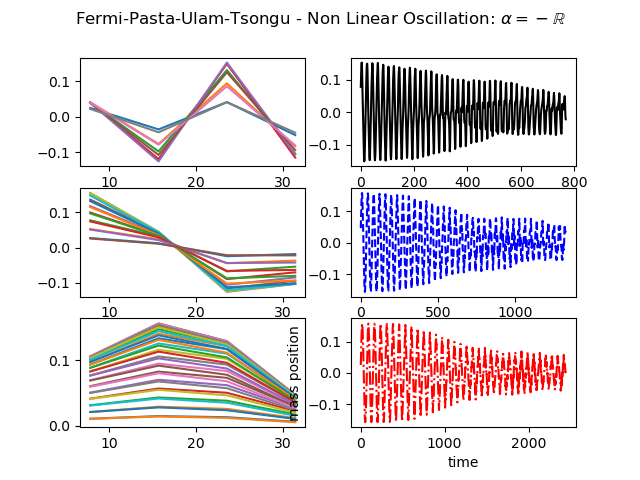
\includegraphics[width=.5\textwidth]{figures/FPUT3.1.png}
\caption{A set of subplots that show the system if we manipulate the system to C = 0.9}
\end{figure}

\begin{figure}[h]
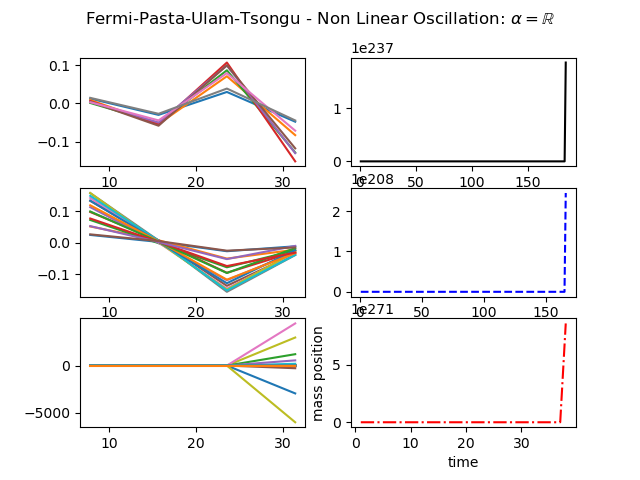
\includegraphics[width=.5\textwidth]{figures/FPUT2.2.png}
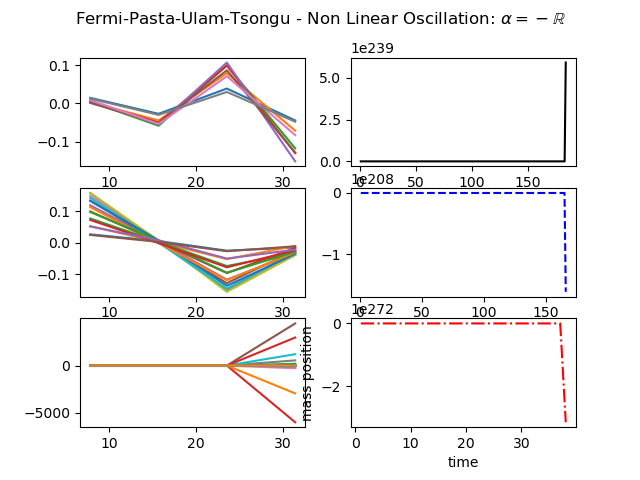
\includegraphics[width=.5\textwidth]{figures/FPUT3.2.png}    
\caption{A set of subplots that show that the system breaks when the value reaches C = 0.99}
\end{figure}

Our last set of experiments that we will run involves this C variable. As it approaches the value 1.0, the solution actually gets ruined. So through some quantative analysis I found a median value for C and tried to see how the behavior of the graphs were affected by this variable. Lets begin with \textbf{Figure 6} and the set of time interval graphs. We can immediatley already see that these graphs in particular are drastically different then our original graphs. We can see as well that all three systems with the different N amount of masses behave differently as well. In our first system we can see that the graogs have apparent local maxima and minima, while the second system has more of a point of intersection. And our last system resembles a figure that almost looks like some surface. In the center mass graph we can see that the oscillations also look very similar. 

As we take a look at our final \textbf{figure 7}, we can see we have officially broken our system. I was able to do this by setting the value inbetweent the interval $0.98 < C < 1.0$. This appears to make total sense because when we were working with the non-linear systems we made it clear that we could no longer use the same time-stepping equation as we did for the linear systems. So as we reach closer and closer to 1.0, we slowly begin to see the time-stepping equation to resemble the previous linear time-stepping equation so it breaks our code. 

\section{Comments}

Through this whole assignment I became more interested in the topic itself. So while I have provided all my findings, and analysis, I wanted to speak shortly about this system and thermalization \cite{therm}. I briefly mentioned in the abstract that the system may reach thermalization which is a process in which mutual interactions cause physical bodies to reach thermal equilibrium. By reaching this equilibrium we are able to see the energy of a system to maximize its entropy \cite{therm2}. Entropy in physics is described as when a physical system hits a state of disorder, or uncertainity. Physicists have been able to calculate this through the equation $S = k_{b} ln \Omega$ \cite{entropy}. This all gets tied back to the Fermi-Pasta-Ulam-Tsingou equation through how the non-linear system behaves. Although the entropy is high for these systems because it has a quasi-period behavior, what we have made an emphasis throughout this paper is that this system has some repeating sequence that cycles over and over and over. With this purpose in mind, I have appreciated the beauty of this system for I have no real scientific reasoning as to why this ODE is the way it is.

\section{Conclusion}

The Fermi-Pasta-Ulam-Tsingou equations are one of the most unqiue systems of ODE's to be discovered to this day. With its unique behavior that is not totally understood, we were able to construct a set of computational tools that allowed us to analyze some of its peculiar behaviors. While I have no academic hypotheses for why this system is the way it is, I thought it was rather interesting to be able to compute this ODE myself. In addition to this research project that we have just conducted, I believe we should give high praise to the four mathematicians who worked with such a system in the 50's. With computational tools being more of a focal point today, it was impressive to see that nearly 70 years ago, Mary Tsingou in particular was able to use scientific computing as a tool to study this equation. So as the power of computation continues to rise exponentially, I am highly curious to continue the mysterious wonders of our natural world.

\section{Acknowledgement}

I just wanted to thank both GSI Ian May, and TA Chris DeGrendele for all their help throughout the Fall 2021 term. I was not only able to grasp a lot of useful computational tools from the both of them, but I got to know two and their intersts in research. I am lucky to have spent time learning from two incredible kind people who have made me become more interested in the field of scientific computing as well. Through this unqiue pandemic university experience they have always made themselves available to help, and I cannot thank them enough for helping me learn more on my young academic journey. Thanks again for a great quarter and as Ian always says Cheers!  

\begin{thebibliography}{15}


\bibitem{Anosov} D.V. Anosov (2001) [1994], "Ergodic theory", Encyclopedia of Mathematics, EMS Press

\bibitem{Quasi} The meteorological glossary: 2d ed. 1930. Meteorological Office, Great Britain. "Certain phenomena which recur more or less regularly but without the exactness of truly periodic phenomena are termed quasi-periodic."

\bibitem{therm} Zabusky, N. J.; Kruskal, M. D. (1965). "Interactions of solitons in a collisionless plasma and the recurrence of initial states". Physical Review Letters. 15 (6): 240–243. Bibcode:1965PhRvL..15..240Z. doi:10.1103/PhysRevLett.15.240

\bibitem{therm2}  "Collisions and Thermalization". sdphca.ucsd.edu. Retrieved 2018-05-14.

\bibitem{entropy}  Wehrl, Alfred (1 April 1978). "General properties of entropy". Reviews of Modern Physics. 50 (2): 221–260. Bibcode:1978RvMP...50..221W. doi:10.1103/RevModPhys.50.221.
\end{thebibliography}

